%==================================================================
% Ini adalah bab 3
% Silahkan edit sesuai kebutuhan, baik menambah atau mengurangi \section, \subsection
%==================================================================

\chapter[METODE PENELITIAN]{\\ METODE PENELITIAN}

\section{Jenis Penelitian}

Penelitian ini menggunakan metode \textit{Research and Development} (R\&D). Menurut \citet{Sugiyono_2013_RnD}, metode R\&D adalah suatu metode penelitian yang digunakan untuk menghasilkan produk tertentu dan menguji keefektifan produk tersebut. Metode ini dipilih karena tujuan utama penelitian ini adalah mengembangkan sebuah produk berupa kerangka kerja perangkat lunak, yaitu \textit{Low-code Extensible Agentic Framework} (LEAF).
Kerangka kerja ini memungkinkan pengguna mendefinisikan dan mengorkestrasi agen AI secara deklaratif melalui manifes YAML/JSON, dengan memanfaatkan protokol standar \textit{Model Context Protocol} (MCP) dan \textit{Agent-to-Agent} (A2A) untuk interoperabilitas.

Proses pengembangan produk dilaksanakan menggunakan model \textit{Waterfall} sebagai siklus hidup pengembangan perangkat lunak, yang diperkenalkan pertama kali oleh \citet{Royce_1970_Waterfall} dan dikembangkan lebih lanjut dalam literatur rekayasa perangkat lunak modern \citep{Pressman_2014_SE, Sommerville_2016_SE}. Model \textit{Waterfall} dipilih dibandingkan model pengembangan lainnya seperti \textit{Agile} karena memiliki alur kerja yang sistematis dah bertahap, serta cocok untuk proyek yang sudah didefinisikan dengan baik dan juga  stabil \citep{Haniva_2023_Waterfall}.

\begin{figure}[ht]
    \centering
    \usetikzlibrary{shapes.geometric, positioning}
    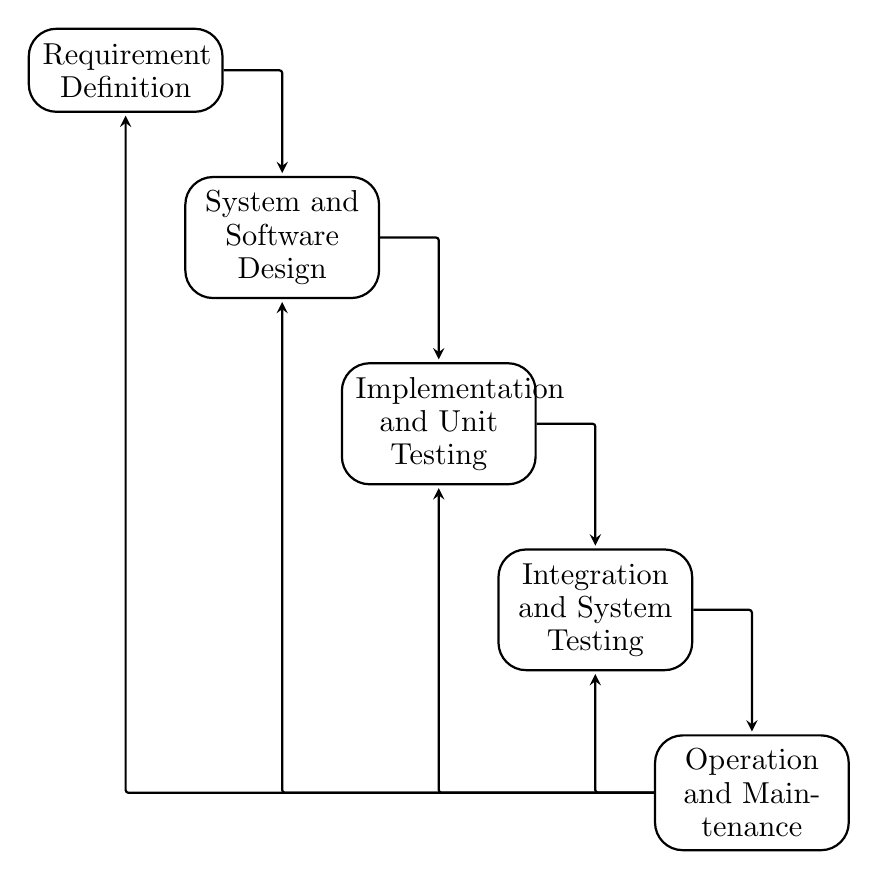
\begin{tikzpicture}[
            node distance=0.8cm and -0.5cm,
            block/.style={
                    rectangle,
                    thick,
                    rounded corners=1em,
                    draw=black,
                    fill=white,
                    align=center,
                    font=\fontsize{10.5}{12}\selectfont,
                    minimum height=3em,
                    minimum width=7em,
                    text width=6em,
                    inner sep=0.5em
                },
            line/.style={
                    draw,
                    thick,
                    ->,
                    >=stealth,
                    shorten >=1pt,
                    rounded corners=1pt
                }
        ]

        % Nodes
        \node [block] (req) {Requirement Definition};
        \node [block, below right=of req] (sys) {System and Software Design};
        \node [block, below right=of sys] (imp) {Implementation and Unit Testing};
        \node [block, below right=of imp] (int) {Integration and System Testing};
        \node [block, below right=of int] (ops) {Operation and Maintenance};

        % Sequential arrows
        \path [line] (req.east) -| (sys.north);
        \path [line] (sys.east) -| (imp.north);
        \path [line] (imp.east) -| (int.north);
        \path [line] (int.east) -| (ops.north);

        % Back arrows
        \path [line] (ops.west) -| (req.south);
        \path [line] (ops.west) -| (sys.south);
        \path [line] (ops.west) -| (imp.south);
        \path [line] (ops.west) -| (int.south);
    \end{tikzpicture}
    \caption{Diagram model \textit{Waterfall}}
    \label{fig:waterfall}
\end{figure}

Pada model ini, terdapat lima tahap yang dilaksanakan secara berurutan: ~(1) \textit{Requirements Definition}, ~(2) \textit{System and Software Design}, ~(3) \textit{Implementation and Unit Testing}, ~(4) \textit{Integration and System Testing}, dan ~(5) \textit{Operation and Maintenance}, sebagaimana yang diilustrasikan pada Gambar~\ref{fig:waterfall}. Masing-masing tahap menghasilkan artefak yang menjadi masukan bagi tahap berikutnya, sehingga tidak memungkinkan melewati salah satu tahap langsung ke tahap selanjutnya. Tahapan yang dilakukan pada penelitian ini terbatas hingga tahap keempat (\textit{Integration and System Testing}), sedangkan tahap kelima (\textit{Operation and Maintenance}) dilakukan ketika nantinya digunakan secara nyata dan terdapat peerkembangan kebutuhan dari pengguna.

\section{Metode Penelitian}

\subsection{\textit{Requirements Definition}}

Tahap \textit{requirements definition} bertujuan untuk mengidentifikasi dan mendokumentasikan kebutuhan fungsional maupun non-fungsional dari LEAF. Pada tahap ini, digunakan metode kuesioner yang ditujukan kepada para ahli \textit{cloud computing}, SRE, \textit{system administrator}, dan peran serupa lainnya untuk mengumpulkan kebutuhan dari perspektif ahli bidang. Kuesioner dirancang untuk mengevaluasi kebutuhan terkait fitur inti kerangka kerja seperti definisi deklaratif, integrasi MCP/A2A, orkestrasi multi-agen, serta kebutuhan non-fungsional seperti interoperabilitas, ekstensibilitas, dan kemudahan penggunaan.

\subsection{\textit{System and Software Design}}

Berdasarkan kebutuhan yang telah diidentifikasi pada tahap sebelumnya, dilakukan tahap \textit{System and Software Design} untuk menerjemahkan kebutuhan tersebut menjadi arsitektur dan spesifikasi teknis LEAF. Proses desain dilakukan dengan pendekatan \textit{top-down}, dimulai dari perancangan arsitektur sistem keseluruhan hingga spesifikasi antarmuka. Aktivitas desain mencakup 2 aspek utama:
\begin{enumerate}[label=\alph*.]
    \item Desain sistem: Perancangan desain sistem yang mencakup arsitektur komponen-komponen utama kerangka kerja, seperti tipe dan hierarki agen, serta aturan kapabilitas masing-masing tipe agen. Desain sistem juga mencakup perancangan pola orkestrasi dan koordinasi multi-agen.
    \item Desain antarmuka: Perancangan antarmuka mencakup antarmuka pengguna serta antarmuka sistem.
          \begin{itemize}
              \item Untuk antarmuka pengguna, meliputi desain format manifes deklaratif (YAML/JSON) untuk mendefinikan agen serta peralatan, dengan fokus pada kemudahan penggunaan dan kejelasan struktur.
              \item Untuk antarmuka sistem meliputi desain komunikasi antar agen dengan protokol A2A, serta desain komunikasi ke server peralatan dengan protokol MCP.
          \end{itemize}
\end{enumerate}

\subsection{\textit{Implementation and Unit Testing}}

Pada tahap \textit{implementation and unit testing} ini, desain pada tahap sebelumnya direalisasikan menjadi kode program kerangka kerja yang fungsional. Implementasi kerangka kerja LEAF pada penelitian ini dilakukan menggunakan bahasa pemrograman Python dan \textit{library} Google ADK yang mendukung integrasi \textit{native} dengan MCP dan A2A. Sedangkan untuk implementasi manifest, dibuat standar format YAML/JSON menggunakan JSON Schema untuk memudahkan validasi struktur manifest bagi pengguna.

\subsection{\textit{Integration and System Testing}}

Pengujian kerangka kerja LEAF pada tahap ini dilakukan dengan metode \textit{black-box}, yaitu dengan mengimplementasikan kerangka kerja LEAF dalam studi kasus pembuatan agen AI untuk bidang \textit{observability} Kubernetes dan operasi SRE. Berdasarkan implementasi tersebut, dilakukan validasi dan evaluasi untuk memastikan bahwa kerangka kerja memenuhi kebutuhan yang telah ditetapkan. Pengujian dilakukan berdasarkan standar kualitas ISO/IEC 25010:2023, dengan pemfokusan pada aspek \textit{Functional Suitability}, \textit{Compatibility}, \textit{Interaction Capability}, and \textit{Flexibility} yang relevan dengan karakteristik produk yang dikembangkan.

\section{Tempat dan Waktu Penelitian}

Penelitian dilakukan di Fakultas Teknik, Universitas Negeri Yogyakarta serta secara daring. Pengembangan kerangka kerja LEAF dan pengujian dilaksanakan menggunakan infrastruktur komputasi awan dan klaster Kubernetes yang dapat diakses secara jarak jauh. Tahapan penelitian secara keseluruhan dilaksanakan dalam jangka waktu bulan Maret--Mei tahun 2026, dengan jadwal yang dipetakan terhadap tahapan model \textit{Waterfall} sebagamana yang dapat diamati pada Tabel~\ref{tab:jadwal}.

\begin{table}[ht]
    \centering
    \caption{Jadwal Pelaksanaan Penelitian}
    \label{tab:jadwal}
    \small
    \begin{tabular}{|l|c|c|c|c|c|c|c|c|c|c|c|c|}
        \hline
        \multirow{2}{*}{\textbf{Kegiatan}}       & \multicolumn{4}{c|}{\textbf{Maret}} & \multicolumn{4}{c|}{\textbf{April}} & \multicolumn{4}{c|}{\textbf{Mei}}                                                                                                             \\
        \cline{2-13}
                                                 & 1                                   & 2                                   & 3                                 & 4         & 1         & 2         & 3         & 4         & 1         & 2         & 3         & 4         \\
        \hline
        \textit{Requirements Definition}         & $\bullet$                           & $\bullet$                           &                                   &           &           &           &           &           &           &           &           &           \\
        \hline
        \textit{System and Software Design}      &                                     & $\bullet$                           & $\bullet$                         & $\bullet$ &           &           &           &           &           &           &           &           \\
        \hline
        \textit{Implementation and Unit Testing} &                                     &                                     &                                   & $\bullet$ & $\bullet$ & $\bullet$ & $\bullet$ & $\bullet$ &           &           &           &           \\
        \hline
        \textit{Integration and System Testing}  &                                     &                                     &                                   &           &           &           &           & $\bullet$ & $\bullet$ & $\bullet$ &           &           \\
        \hline
        Penyusunan Laporan                       & $\bullet$                           & $\bullet$                           & $\bullet$                         & $\bullet$ & $\bullet$ & $\bullet$ & $\bullet$ & $\bullet$ & $\bullet$ & $\bullet$ & $\bullet$ & $\bullet$ \\
        \hline
    \end{tabular}
\end{table}

\section{Subjek Penelitian}

Subjek penelitian ini terdiri dari para ahli yang berperan sebagai validator dan evaluator untuk hasil pengembangan kerangka kerja LEAF serta implementasinya dalam studi kasus \textit{observability} Kubernetes dan operasi SRE. Pengujian dilakukan terhadap aspek \textit{Functional Suitability}, \textit{Compatibility}, \textit{Interaction Capability}, dan \textit{Flexibility} yang telah ditetapkan kepada 5 responden ahli terpilih. Pemilihan responden ahli didasarkan pada latar belakang profesional dan pengalaman mereka dalam bidang terkait, yaitu praktisi \textit{cloud computing}, SRE, \textit{system administrator}, dan peran serupa lainnya.

\section{Metode Pengumpulan Data}

Data yang dikumpulkan dalam penelitian pengembangan kerangka kerja LEAF ini terdiri dari data primer dan data sekunder. Metode pengumpulan data yang digunakan adalah sebagai berikut.

\subsection{Studi Pustaka}

Studi pustaka dilakukan untuk mengumpulkan data sekunder berupa teori, konsep, dan temuan dari penelitian-penelitian terdahulu yang relevan. Sumber pustaka meliputi jurnal ilmiah internasional, buku teks, dokumentasi teknis standar (seperti protokol A2A dan MCP), dan publikasi dari organisasi seperti CNCF dan Linux Foundation. Hasil studi pustaka menjadi dasar untuk menetapkan kebutuhan kerangka kerja pada tahap \textit{Requirement Analysis}.

\subsection{Kuesioner}

Kuesioner digunakan untuk mengumpulkan data primer dari para ahli terkait kebutuhan dan fitur yang diharapkan dari kerangka kerja LEAF pada tahap  \textit{Requirement Analysis}, serta untuk mengumpulkan data validasi dan evaluasi dari para ahli setelah pengembangan produk pada tahap \textit{Integration and System Testing}. Kuesioner dirancang dengan menggunakan skala Likert untuk menilai tingkat kebutuhan dan kepuasan terhadap fitur-fitur yang dikembangkan, serta untuk mengidentifikasi potensi peningkatan berdasarkan masukan dari para ahli.

\subsection{Wawancara}

Wawancara dilakukan secara mendalam dengan beberapa responden ahli untuk mendapatkan pemahaman yang lebih komprehensif tentang kebutuhan, tantangan, dan harapan mereka terkait pengembangan kerangka kerja LEAF. Wawancara dilakukan secara daring menggunakan platform komunikasi pertemuan video, dengan panduan wawancara yang telah disiapkan sebelumnya untuk memastikan konsistensi dalam pengumpulan data. Wawancara ini juga digunakan untuk menggali lebih dalam tentang masukan yang diberikan dan mendapatkan wawasan tambahan yang mungkin tidak terungkap melalui kuesioner.

\section{Instrumen Penelitian}

Instrumen penelitian disusun berdasarkan tujuan penelitian dan kebutuhan pengumpulan data, yang digunakan untuk memvalidasi dan mengevaluasi kerangka kerja LEAF. Instrumen yang digunakan dalam penelitian ini dikembangkan berdasarkan aspek \textit{Functional Suitability}, \textit{Compatibility}, \textit{Interaction Capability}, dan \textit{Flexibility} dari standar ISO/IEC 25010:2023 yang relevan dengan karakteristik produk yang dikembangkan. Dalam praktik pengujiannya, instrumen disusun dalam bentuk kuesioner/lembar penilaian yang dikembangkan mengikuti pendekatan \citet{Arikunto_2013_Prosedur}. Lembar penilaian menggunakan skala Likert lima tingkat untuk menilai setiap indikator. Skala penilaian yang digunakan disajikan pada Tabel~\ref{tab:skala}.

\begin{table}[ht]
    \centering
    \caption{Skala Penilaian Instrumen Kuesioner}
    \label{tab:skala}
    \begin{tabular}{|c|l|l|}
        \hline
        \textbf{Skor} & \textbf{Kategori} & \textbf{Keterangan}                               \\
        \hline
        5             & Sangat Baik       & Sepenuhnya sesuai dan tanpa kekurangan            \\
        \hline
        4             & Baik              & Sebagian besar sesuai dengan sedikit kekurangan   \\
        \hline
        3             & Cukup             & Cukup sesuai namun memerlukan perbaikan           \\
        \hline
        2             & Kurang            & Kurang sesuai dan memerlukan perbaikan signifikan \\
        \hline
        1             & Sangat Kurang     & Tidak sesuai dan perlu perancangan ulang          \\
        \hline
    \end{tabular}
\end{table}


% \subsection{\textbf{Fungsionalitas (\textit{Functionality})}}

% Kesesuaian fitur dengan kebutuhan, kelengkapan fitur inti (definisi agen deklaratif, integrasi MCP/A2A, orkestrasi multi-agen), dan kebenaran fungsional.

% \subsection{\textbf{Kegunaan (\textit{Usability})}}

% Kemudahan penggunaan manifes deklaratif, kejelasan dokumentasi, kurva pembelajaran, dan pengalaman pengguna dalam mendefinisikan agen tanpa pemrograman.

% \subsection{\textbf{Keandalan (\textit{Reliability})}}

% Konsistensi perilaku \textit{framework}, penanganan kesalahan, dan stabilitas pada berbagai skenario penggunaan.

% \subsection{\textbf{Pemeliharaan (\textit{Maintainability})}}

% Kualitas kode, modularitas arsitektur, kemudahan perluasan (\textit{extensibility}), dan kesesuaian dengan standar.

\subsection{Instrumen \textit{Functional Suitability}}

Instrumen untuk mengukur \textit{Functional Suitability} dirancang untuk mengevaluasi sejauh mana fitur-fitur yang dikembangkan memenuhi kebutuhan fungsional yang telah ditetapkan. Indikator yang digunakan meliputi kesesuaian fitur dengan kebutuhan, kelengkapan fitur inti (definisi agen deklaratif, integrasi MCP/A2A, orkestrasi multi-agen), dan kebenaran fungsional.

\subsection{Instrumen \textit{Compatibility}}

Instrumen untuk mengukur \textit{Compatibility} dirancang untuk mengevaluasi sejauh mana kerangka kerja LEAF dapat beroperasi dengan baik dalam lingkungan yang berbeda, serta kemampuannya untuk berinteraksi dengan sistem dan perangkat lunak lain. Indikator yang digunakan meliputi interoperabilitas dengan protokol standar, kemampuan integrasi dengan berbagai platform, dan kompatibilitas dengan berbagai jenis agen dan peralatan.

\subsection{Instrumen \textit{Interaction Capability}}

Instrumen untuk mengukur \textit{Interaction Capability} dirancang untuk mengevaluasi sejauh mana kerangka kerja LEAF dapat mendukung interaksi yang efektif antara agen, serta antara agen dengan pengguna. Indikator yang digunakan meliputi kemampuan komunikasi antar agen, kemampuan beradaptasi dengan konteks interaksi, dan kemudahan penggunaan antarmuka untuk mendefinisikan interaksi.

\subsection{Instrumen \textit{Flexibility}}

Instrumen untuk mengukur \textit{Flexibility} dirancang untuk mengevaluasi sejauh mana kerangka kerja LEAF dapat dengan mudah disesuaikan dan diperluas untuk memenuhi kebutuhan yang berubah. Indikator yang digunakan meliputi kemudahan dalam menambahkan fitur baru, kemampuan untuk menyesuaikan perilaku agen, dan kemampuan untuk beradaptasi dengan berbagai skenario penggunaan.

\section{Teknik Analisis Data}

Teknik analisis data yang digunakan dalam penelitian ini disesuaikan dengan jenis data yang dikumpulkan, yaitu data kuantitatif dari instrumen validasi dan pengujian, serta data kualitatif dari masukan para ahli.

\subsection{Analisis Deskriptif untuk Validasi Ahli}

Data kuantitatif dari lembar validasi ahli dianalisis secara deskriptif menggunakan perhitungan persentase kelayakan. Persentase kelayakan dihitung dengan rumus:

\begin{equation}
    \text{Persentase Kelayakan} = \frac{\text{Skor yang diperoleh}}{\text{Skor maksimal}} \times 100\%
    \label{eq:kelayakan}
\end{equation}

Hasil perhitungan persentase kelayakan kemudian diinterpretasikan berdasarkan klasifikasi kelayakan yang disajikan pada Tabel~\ref{tab:kelayakan}.

\begin{table}[ht]
    \centering
    \caption{Klasifikasi Kelayakan Produk}
    \label{tab:kelayakan}
    \begin{tabular}{|c|l|}
        \hline
        \textbf{Persentase} & \textbf{Kategori Kelayakan} \\
        \hline
        81\% -- 100\%       & Sangat Layak                \\
        \hline
        61\% -- 80\%        & Layak                       \\
        \hline
        41\% -- 60\%        & Cukup Layak                 \\
        \hline
        21\% -- 40\%        & Kurang Layak                \\
        \hline
        0\% -- 20\%         & Tidak Layak                 \\
        \hline
    \end{tabular}
\end{table}

Produk dinyatakan layak untuk digunakan apabila persentase kelayakan dari seluruh aspek penilaian mencapai kategori minimal ``Layak'' (61\%). Jika terdapat aspek yang memperoleh kategori di bawah ``Layak'', maka dilakukan revisi pada aspek tersebut dan validasi ulang hingga kriteria kelayakan terpenuhi.

\subsection{Analisis Pengujian Fungsional}

Data dari pengujian fungsional dianalisis berdasarkan persentase keberhasilan kasus uji. Setiap kasus uji menghasilkan dua kemungkinan hasil: berhasil (\textit{pass}) atau gagal (\textit{fail}). Persentase keberhasilan dihitung dengan rumus:

\begin{equation}
    \text{Persentase Keberhasilan} = \frac{\text{Jumlah kasus uji berhasil}}{\text{Total kasus uji}} \times 100\%
    \label{eq:keberhasilan}
\end{equation}

\textit{Framework} dinyatakan memenuhi kebutuhan fungsional apabila seluruh kasus uji (100\%) berhasil dieksekusi sesuai keluaran yang diharapkan. Jika terdapat kasus uji yang gagal, dilakukan identifikasi penyebab kegagalan, perbaikan kode, dan pengujian ulang hingga seluruh kasus uji berhasil.

\subsection{Analisis Kualitatif}

Data kualitatif berupa komentar, saran, dan masukan dari para ahli validator dianalisis melalui proses berikut:
\begin{enumerate}
    \item \textbf{Pengumpulan dan pencatatan}: Seluruh komentar dan saran dari para ahli dikumpulkan dan dicatat secara sistematis.
    \item \textbf{Kategorisasi}: Masukan dikategorikan berdasarkan aspek yang dibahas (fungsionalitas, kegunaan, keandalan, atau pemeliharaan) dan tingkat urgensi (kritis, penting, atau saran).
    \item \textbf{Prioritisasi}: Masukan diprioritaskan berdasarkan dampaknya terhadap kualitas \textit{framework}. Masukan kritis dan penting diprioritaskan untuk ditindaklanjuti segera.
    \item \textbf{Implementasi revisi}: Perbaikan dilakukan pada \textit{framework} berdasarkan masukan yang telah diprioritaskan.
    \item \textbf{Dokumentasi perubahan}: Setiap perubahan yang dilakukan berdasarkan masukan ahli didokumentasikan untuk pelacakan dan akuntabilitas.
\end{enumerate}

Kombinasi analisis kuantitatif dan kualitatif memberikan evaluasi yang komprehensif terhadap kualitas produk, memungkinkan penilaian numerik yang objektif sekaligus pemahaman mendalam tentang aspek-aspek yang memerlukan perbaikan.